\documentclass[a4paper]{article}
\usepackage[italian]{babel}
\usepackage[utf8]{inputenc}
\usepackage[T1]{fontenc}
\usepackage{float}
\usepackage{hyperref}
\usepackage{graphicx}
\usepackage{fancyvrb}
\usepackage{fvextra}
\usepackage{csquotes}
\usepackage[backend=biber, style=ieee]{biblatex}
\usepackage{glossaries}
\addbibresource{bibliografia.bib}

\title{Relazione di progetto di Virtualizzazione e integrazione di sistemi\\
\textbf{Server NFS e volumi di container}}
\date{\today}
\author{Luca Casadei\\Matricola: 0001069237}
\makeglossaries

\loadglsentries{defns}
\setacronymstyle{short-long}

\begin{document}
\maketitle

\tableofcontents

\section{Creazione delle macchine virtuali}
In questa sezione verrà indicata la modalità utilizzata per la creazione delle macchine virtuali, 
in particolar modo verrà descritto il modo usato per metterle in comunicazione.
\subsection{Ambiente di virtualizzazione}
Come ambiente di virtualizzazione è stato scelto \textit{Proxmox}, un software debian-based open source che permette di gestire macchine virtuali basato
sull'infrastruttura \gls{KVM} che fornisce già un repository di immagini \gls{LXC}.
\\
Procedo quindi ad un'installazione "fresca" di Proxmox su una workstation, a seguito di tutte le fasi di installazione, mi trovo nella seguente situazione:
\begin{figure}[H]
    \centering
    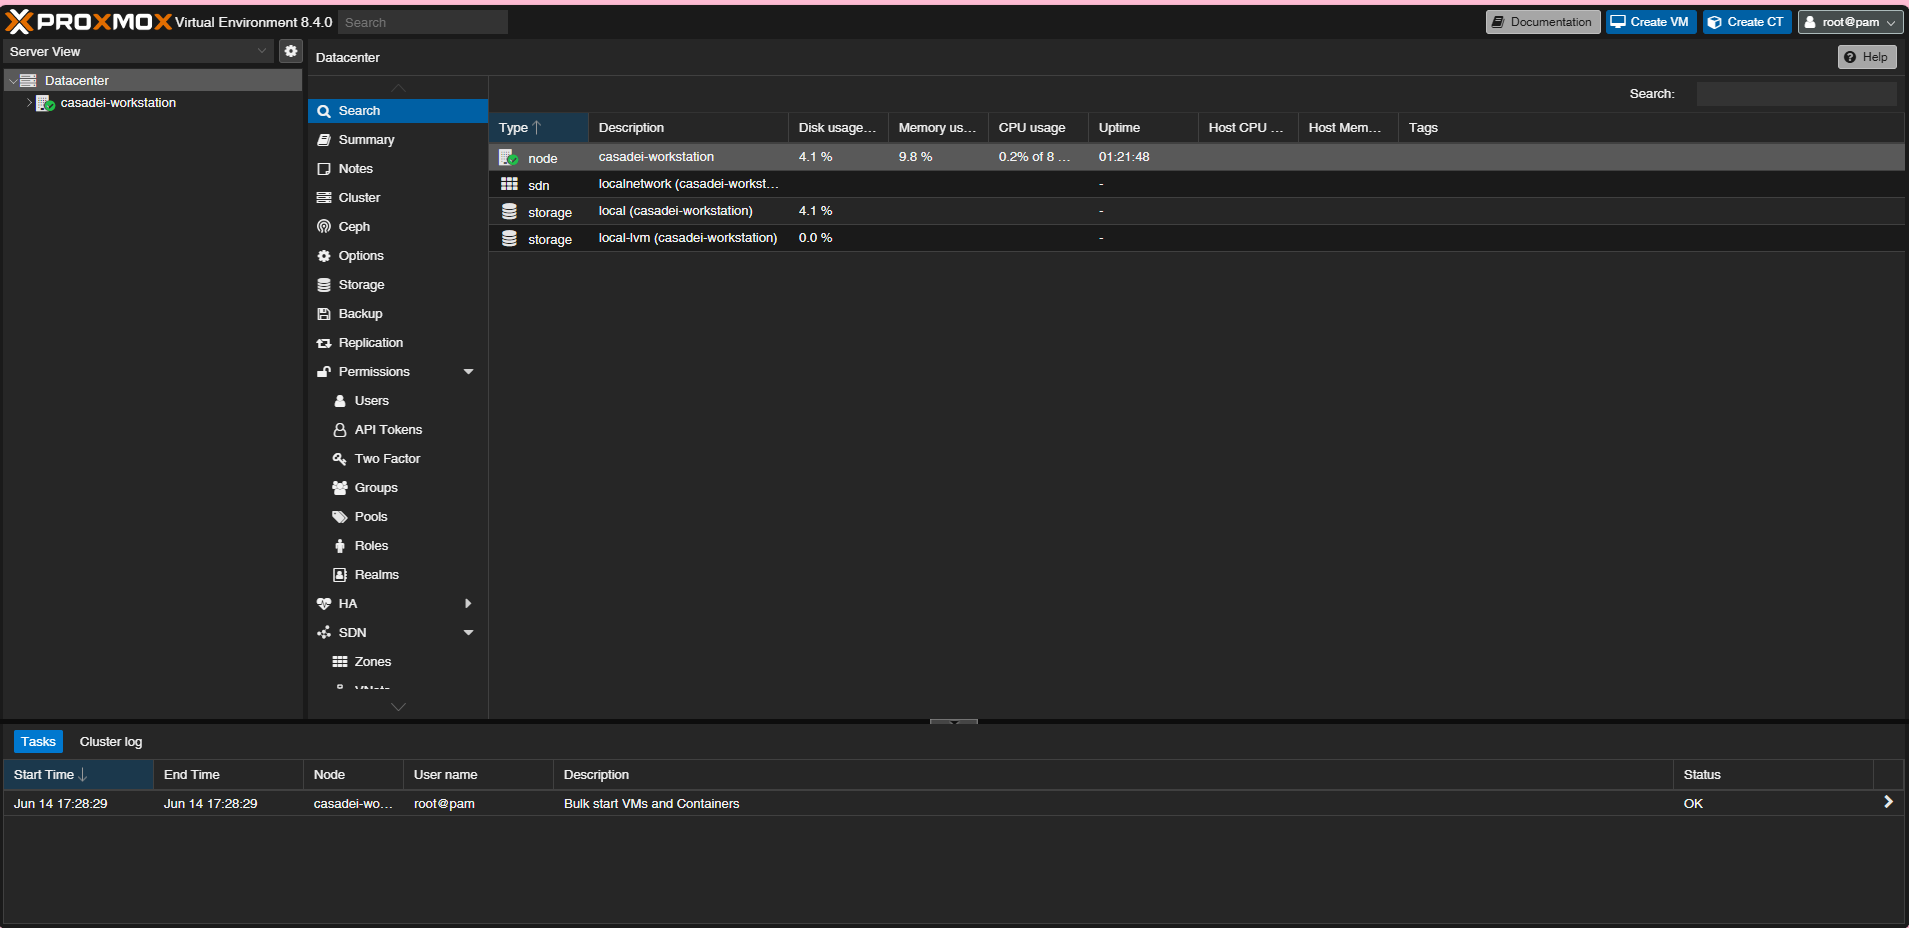
\includegraphics[scale=0.22]{images/ProxMoxDopoInstallazione.png}
    \caption{Proxmox installato su workstation}
\end{figure}

\subsection{Creazione server NFS}
\subsubsection{Cenni su NFS e NFSv4}
Il protocollo \Gls{NFS} versione 4 descritto dalla \cite[rfc7530]{rfc7530} è un'evoluzione dello stesso protocollo in versione 3 e 2 descritti
rispettivamente dalle \cite[rfc1813]{rfc1813} e \cite[rfc1094]{rfc1094}, l'idea alla base del protocollo è quella di rendere accessibile delle
risorse (file) all'interno della rete, indipendentemente dal sistema operativo o architettura di rete. Per realizzare questa astrazione il protocollo
fa uso di primitive chiamate \Gls{RPC} ed una rappresentazione dei dati esterna a quella dei vari sistemi operativi, ma interpretabile da tutti attraverso
la rete, la \Gls{XDR}.\\
NFS era (originariamente) pensato per essere un protocollo stateless, quindi non manteneva informazioni riguardanti i client che ne facevano uso. La versione 2 introduce la possibilità
di gestire file di dimensioni notevolmente superiori rispetto alla versione precedente, oltre all'introduzione di nuove primitive e migliorie a livello di
integrità dei dati in caso di operazioni asincrone.\\
Dalla versione 4, con l'introduzione del file locking (modalità per irrobustire l'integrità dei file trasferiti) il protocollo è necessariamente diventato stateful, rendendo quindi
incompatibili il protocollo in versione 4 e le versioni precedenti, nonostante questo gran parte dei server nfs consentono di configurare il protocollo in più versioni diverse. 

\subsubsection{Effettiva crazione}
Ora andrò a creare la macchina virtuale che conterrà il container per il server NFSv4, non uso un container LXC Proxmox
perché NFSv4 richiede accesso kernel-level. Come sistema da virtualizzare ho scelto Debian 12, che scarico e aggiungo alle ISO
Images di Proxmox (nell'hdd secondario), con il seguente risultato:
\begin{figure}[H]
    \centering
    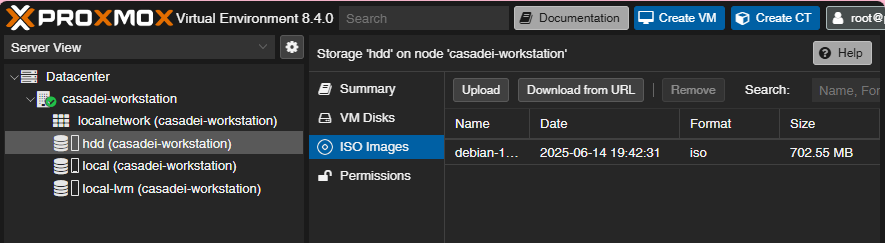
\includegraphics[scale=0.42]{images/IsoDebian12Caricata1.png}
    \caption{Aggiunta ISO Debian 12 a Proxmox}
\end{figure}
Ora procedo a creare la macchina virtuale effettiva seguendo tutte le configurazioni di
Proxmox, questa è la finestra di creazione finalizzata:
\begin{figure}[H]
    \centering
    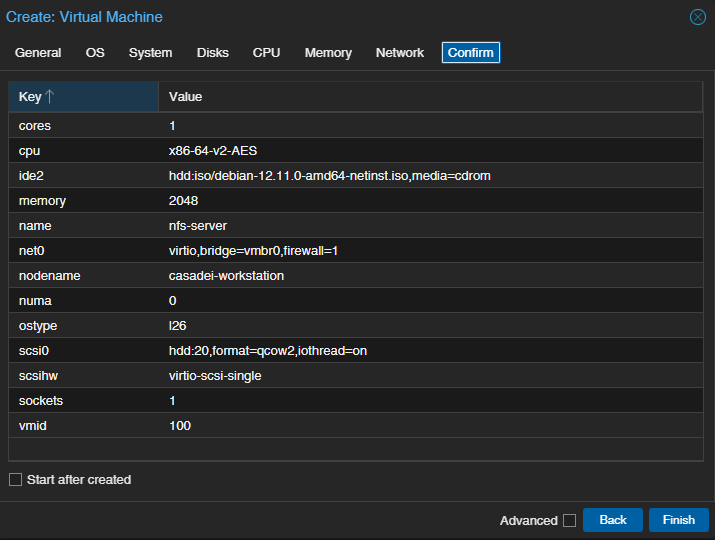
\includegraphics[scale=0.60]{images/VMNFSServer.png}
    \caption{Creazione della macchina virtuale per il server NFSv4}
\end{figure}
Si procede quindi all'installazione di Debian normale, a seguito dell'avvio della macchina
virtuale, dopodiché procedo ad installare tutti i pacchetti necessari, a partire da docker:
\subsubsection{Installazione di Docker Engine e Compose}
Dalla documentazione ufficiale di Docker, aggiungiamo la chiave \Gls{GPG}
per poter installare il pacchetto:
\begin{Verbatim}[numbers=left,breaklines]
    # Add Docker's official GPG key:
    sudo apt-get update
    sudo apt-get install ca-certificates curl
    sudo install -m 0755 -d /etc/apt/keyrings
    sudo curl -fsSL https://download.docker.com/linux/debian/gpg -o /etc/apt/keyrings/docker.asc
    sudo chmod a+r /etc/apt/keyrings/docker.asc

    # Add the repository to Apt sources:
    echo \
    "deb [arch=$(dpkg --print-architecture) signed-by=/etc/apt/keyrings/docker.asc] https://download.docker.com/linux/debian \
    $(. /etc/os-release && echo "$VERSION_CODENAME") stable" | \
    sudo tee /etc/apt/sources.list.d/docker.list > /dev/null
    sudo apt-get update
\end{Verbatim}
E installimo i pacchetti:
\begin{Verbatim}[numbers=left,breaklines]
    sudo apt-get install docker-ce docker-ce-cli containerd.io docker-buildx-plugin docker-compose-plugin
\end{Verbatim}
provando ad eseguire il comando:
\begin{Verbatim}[numbers=left]
    docker ps
\end{Verbatim}
otteniamo:
\begin{figure}[H]
    \centering
    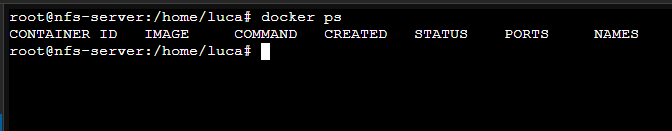
\includegraphics[scale=0.65]{images/DockerInstallato.png}
    \caption{Output di Docker PS dopo averlo installato}
\end{figure}
\subsubsection{Creazione e configurazione del container nfs-server}
Abilitiamo i moduli NFS e NFSD dal kernel linux:
\begin{Verbatim}[numbers=left,breaklines]
    sudo modprobe {nfs,nfsd}
\end{Verbatim}
in alternativa si possono aggiungere questi due moduli nel file \textit{/etc/modules}
Come immagine per docker verrà utilizzata \href{https://hub.docker.com/r/erichough/nfs-server/}{\textbf{nfs-server}}
e verrà configurata mediante lo script compose chiamato: "nfs-docker-compose.yml" (Vedi file per dettagli)
Dopo aver creato lo script ed eseguito "docker compose up" per farlo partire, nfs-server dovrebbe darci il seguente output:
\begin{figure}[H]
    \centering
    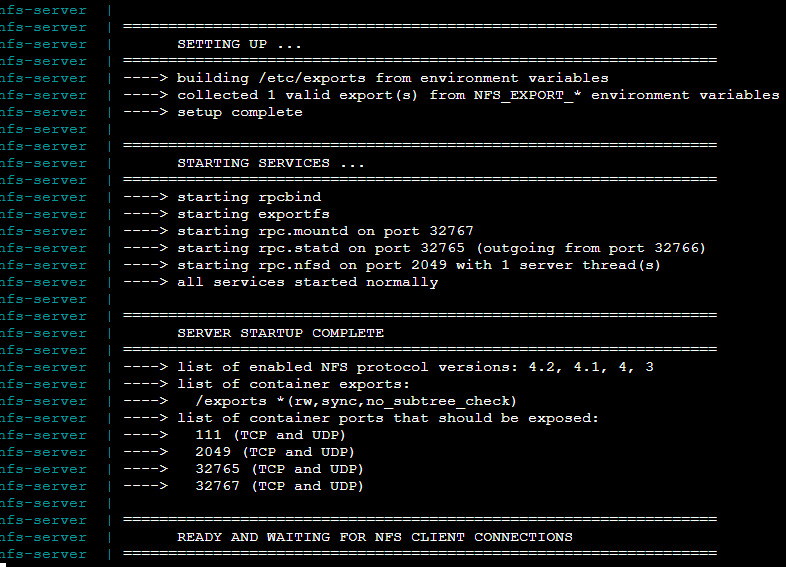
\includegraphics[scale=0.30]{images/NFSSettato.png}
    \caption{Dopo docker compose up}
\end{figure}

\subsection{Creazione della seconda macchina virtuale (WebServer)}
\subsubsection{Sistema operativo}
Come sistema operativo della seconda macchina virtuale ho scelto \textit{Alpine Linux} per due ragioni principali, la prima
è per mostrare il funzionamento anche su sistemi leggermente diversi, seppur entrambi linux, e questo è estremamente leggero e minimale,
la seconda ragione è una personale avversione ad installare sistemi non open source. Questa è la configurazione della macchina virtuale,
con un processore Intel.

\begin{figure}[H]
    \centering
    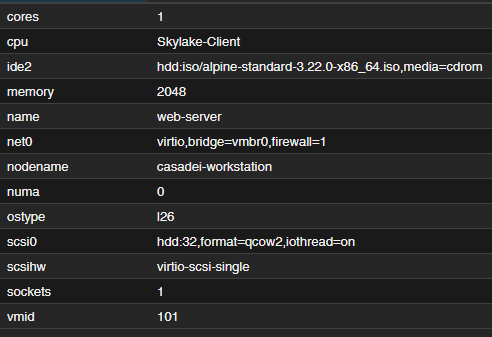
\includegraphics[scale=0.9]{images/VMWebServer.png}
    \caption{Creazione della macchina virtuale per il WebServer}
\end{figure}

Si procede quindi all'installazione su disco di Alpine Linux mediante il comando \textit{"setup-alpine"},
per verificare la corretta impostazione delle interfacce con dhcp si può usare \textit{"ip a"} 
e si ottiene:
\begin{figure}[H]
    \centering
    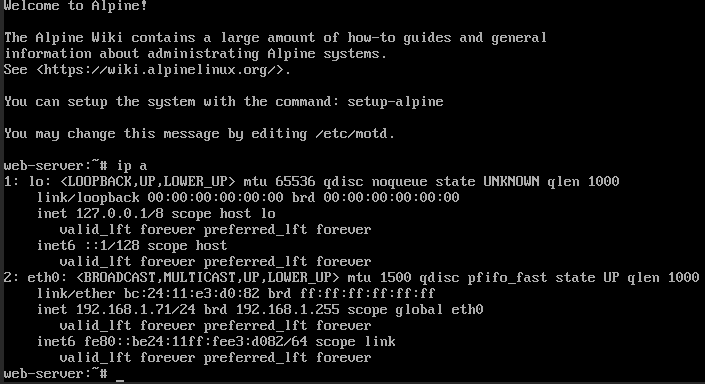
\includegraphics[scale=0.6]{images/AlpineInstallato.png}
    \caption{Alpine Linux installato}
\end{figure}

\subsubsection{Comunicazione tra macchine virtuali}
Tornando alla prima macchina virtuale e lanciando un ping, si può vedere che le due macchine riescono a 
comunicare.
\begin{figure}[H]
    \centering
    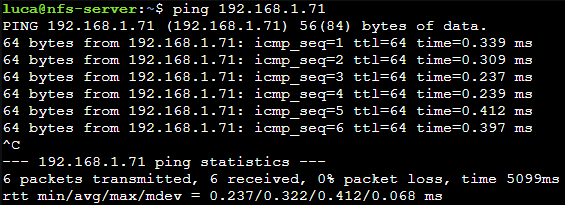
\includegraphics[scale=0.8]{images/MacchineComunicano.png}
    \caption{I due server comunicano con ping}
\end{figure}
Se vogliamo usare i nomi di dominio, essendo il bridge di proxmox assegnato alle macchine virtuali di default (vmbr0)
condiviso con la rete della macchina host (la workstation), la configurazione di rete viene data dal router a cui è collegata
la workstation mediante DHCP, e se il router funge anche da server DNS, ci consente di trovare nella rete locale le macchine (virtuali o no)
mediante il loro nome di dominio, ottenendo quindi il seguente risultato con ping:
\begin{figure}[H]
    \centering
    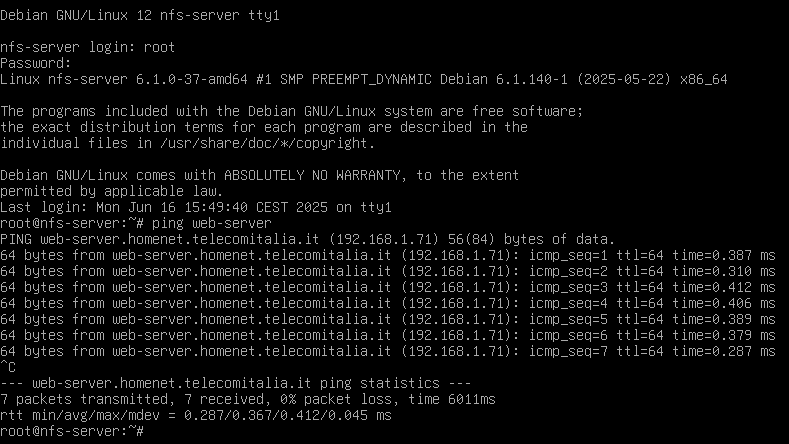
\includegraphics[scale=0.55]{images/MacchineComunicanoHostname.png}
    \caption{Macchine comunicano anche usando hostname}
\end{figure}
Se questo non fosse possibile, potremmo modificare il file \textit{"/etc/hosts"} all'interno delle macchine virtuali ed aggiungere manualmente il
nome di dominio, ad esempio, questo potrebbe essere il file hosts all'interno della macchina nfs-server che contiene il record dell'altra macchina virtuale:
\begin{figure}[H]
    \centering
    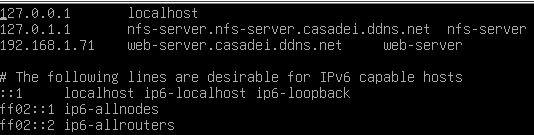
\includegraphics[scale=0.8]{images/HostsNfs.png}
    \caption{File hosts in /etc nella macchina nfs-server}
\end{figure}
se usiamo ping adesso, in nome di dominio completo sarà diverso da quello precedente perché non è più quello fornito dal server dns del router:
\begin{figure}[H]
    \centering
    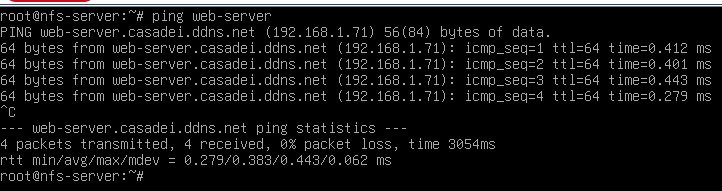
\includegraphics[scale=0.60]{images/HostsNFSPing.png}
    \caption{Nome di dominio diverso se in file hosts}
\end{figure}
Un'ulteriore alternativa sarebbe quella di creare (virtuale o meno) un server DNS all'interno della stessa rete per evitare di andare ad aggiungere ogni
hostname nel file /etc/hosts di ogni macchina, sarebbe la soluzione più raffinata ma il procedimento per questa modalità verrà omesso perché non rientrante
nell'obiettivo del progetto.

\subsubsection{Prova specifica NFS}
Ora facciamo però una prova specifica con NFS, dopo aver installato su alpine nfs-utils (solo per prova, non servirà nel sistema finale)
possiamo montare un percorso connettendoci al server NFS, con i comandi visibili nell'immagine, e successivamente creare un file in una delle
due cartelle predisposte per l'esportazione dal server NFS, ad esempio "db":
\begin{figure}[H]
    \centering
    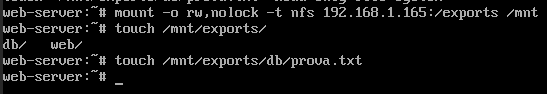
\includegraphics[scale=0.8]{images/ProvaNFS.png}
    \caption{Mount del percorso esposrtato e creazione di file di prova}
\end{figure}
Questo file deve ora essere visibile anche dal server, nella corrispondente cartella:
\begin{figure}[H]
    \centering
    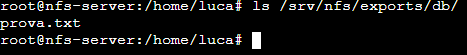
\includegraphics[scale=0.9]{images/NFSFunziona.png}
    \caption{file visibile nel server NFS}
\end{figure}
\section{Creazione di un servizio che si appoggia su volumi NFS per la persistenza}
Questa è la parte cruciale del progetto, la creazione di un insieme di container che adottino
persistenza dei dati sul nostro server NFS, partiamo quindi dalla creazione del file compose
che metta in esecuzione un semplicissimo e basilare sito web, ed il relativo database, i cui dati
devono essere persistenti e appunto, su volumi NFS.
\subsection{Creazione del sito web di prova e database}
Questi codici sono consultabili dalla repository, non essendo questo progetto incentrato sulla programmazione
web verranno omessi i passaggi per realizzarli in questa relazione, elenco brevemente le tecnologie usate:
\begin{itemize}
    \item \textbf{MariaDB}: Database per testare la persistenza dei dati su volumi NFS
    \item \textbf{PHP}: Lato server
    \item \textbf{Javascript + HTML}: con Apache come server http
\end{itemize}
Il sito presenta un semplice elenco di elementi a caso che si possono aggiungere mediate apposito form, nulla di più.
Il database viene inizialmente popolato dallo script crea-tabella.sql montato come volume di tipo bind durante l'inizializzazione
del container, dato che abbiamo la persistenza dei dati tramite NFS, se vogliamo svuotare completamente il database e forzare di nuovo
l'inizializzazione dobbiamo rimuovere i file che MariaDB crea all'interno della cartella condivisa, o dal server NFS o dal container stesso.
Il container per PHP e Apache viene creato secondo l'apposito Dockerfile corredato assieme alla relazione nella cartella web/sito.
\subsection{Test conclusivo}
Quando lanciamo "docker compose up -d" partendo da web-docker-compose.yml si ottiene:
\begin{figure}[H]
    \centering
    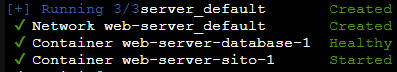
\includegraphics[scale=1]{images/ServiziFunzionanti.png}
    \caption{Servizi funzionanti}
\end{figure}
A questo punto è possibile accedere al sito mediante l'indirizzo della macchina virtuale web-server:
\begin{figure}[H]
    \centering
    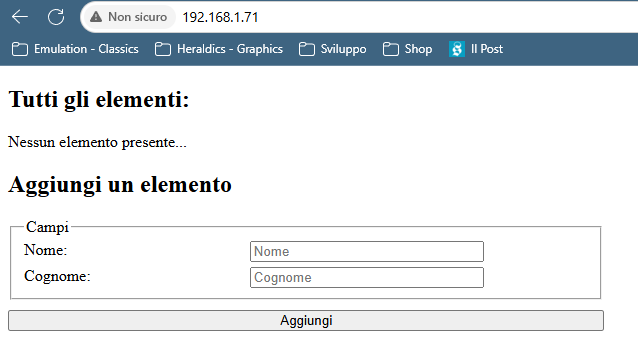
\includegraphics[scale=0.7]{images/PaginaSito.png}
    \caption{Sito web}
\end{figure}
Dal form si possono quindi aggiungere diversi elementi che verranno visualizzati nella lista, per testare la persistenza dei dati, si può forzare il build
del container del database aggiungendo \textit{--build} a docker compose up, e si noterà che gli elementi che erano stati inseriti in precedenza sono ancora
visualizzabili nella lista perché MariaDB vede che ci sono degli elementi pre-esistenti nel volume nfs, se invece si cancellano i file creati da maria db nel volume nfs da un'altra macchina virtuale (o il container stesso) al prossimo
avvio MariaDB dovrà rieffettuare l'inizializzazione, svuotando di conseguenza tutto il suo contenuto, al che alla riapertura del sito non si vedranno più elementi nella lista.
\section{Conclusioni}
\subsection{Struttura del progetto e password}
\begin{itemize}
    \item \textbf{Ambiente di virtualizzazione}: ProxMox
    \begin{itemize}
        \item \textbf{Macchina virtuale 1 (100)}: Contiene container per il server NFS, il percorso dei file è /home/luca, la password per gli account (luca, root) è: nfs
        \item \textbf{Macchina virtuale 2 (101)}: Contiene i servizi web e database che usa volume NFS, il percorso dei file è "/root/servizi/*", la password per gli account (luca, root) è: web-server
        \begin{itemize}
            \item \textbf{web-server}: Container con immagine PHP-Apache creato mediante Dockerfile, il percorso interessato è sito/*
            \item \textbf{database}: Container con immagine MariaDB che monta un volume con driver NFS, il percorso interessato è sql/*
        \end{itemize}
    \end{itemize}
\end{itemize}
Entrambe le macchine hanno accesso ssh abilitato sull'account "luca" con password nfs e web-server


\printglossaries
\printbibliography
\end{document}